%\section{Quickstart Guide}
% The quickstart guide should explain in simple terms and with examples
% how a user is supposed to achieve the most common usecases. E.g. how
% to submit and cancel a job, how to receive a job's output. How to
% create a grid file, move it around, locate it, and delete it. How to
% monitor the progress on an application etc.

This section briefly explains the sequence of operations, from the client configuration, to the description of the 
request up to the retrieval of the generated output, to be performed by a user to have his application run on a 
grid resource.
 

\subsection{Configuration}

Configuration of the WMS User Interface VO-specific parameters is accomplished through the file:

\smallskip
\begin{verbatim}
$GLITE_LOCATION/etc/<vo name>/glite_wmsui.conf 
\end{verbatim}
\smallskip

i.e. there is one directory and file for each supported VO.

If you wish to add a new VO among the ones supported by the WMS-UI, you must create a directory in \$GLITE\_LOCATION/etc, 
named as the VO (lower-case), copy in it the file: 

\smallskip
\begin{verbatim}
$GLITE_LOCATION/etc/vo_template/glite_wmsui.conf 
\end{verbatim}
\smallskip

distributed with the WMS-UI package and update it according to the given VO.

Here follows an example of WMS-UI configuration file for the "EGEE" Virtual Organisation. 
This implies that the file path has to be \emph{\$GLITE\_LOCATION/etc/egee/glite\_wmsui.conf}: 

\smallskip
\begin{verbatim}

[
 VirtualOrganisation = "EGEE";
 NSAddresses = {
   "tigerman.cnaf.infn.it:7772",
   "gundam.cnaf.infn.it:7772"
   };
 LBAddresses = {
   {"tigerman.cnaf.infn.it:9000", "fox.to.infn.it:9000"},
   {"gundam.cnaf.infn.it:9000", "neo.datamat.it:9000", "grid003.ct.infn.it:9876"}
  };
 MyProxyServer = "skurut.cesnet.cz";
 LoggingDestination = "localhost:9002";  // local instance of LB logging service
]

\end{verbatim}
\smallskip

This files indicates that there are two available Network Servers that can be contacted for the EGEE VO (they
are chosen randomly by the WMS-UI) and each NS has a group of associated LB servers:

\begin{itemize}
   \item tigerman.cnaf.infn.it:7772 is associated with tigerman.cnaf.infn.it:9000 and 
fox.to.infn.it:9000
   \item gundam.cnaf.infn.it:9000 is associated with gundam.cnaf.infn.it:9000, neo.datamat.it:9000 
and grid003.ct.infn.it:9876
\end{itemize}

Given a NS the WMS-UI chooses randomly the LB from the corresponding list. This feature can be used to
distribute load over several LB servers, although in most of cases there is a one-to-one correspondence
between NS and LB.

The \emph{MyProxyServer} parameter provides the host FQDN (fully qualified host name) of the MyProxy server 
to be used for proxy renewal (see \ref{longjob}) whilst \emph{LoggingDestination} has to be set in case of 
non-standard location of the LB locallogger (it usually runs on the WMS node). 

The other configuration file for the WMS-UI is

\smallskip
\begin{verbatim}
$GLITE_LOCATION/etc/glite_wmsui_cmd_var.conf
\end{verbatim}
\smallskip

The glite\_wmsui\_cmd\_var.conf file is a class-ad containing information that are not VO specific. 

\textbf{Example:}
\smallskip
\begin{verbatim}
[ 
 requirements = other.GlueCEStateStatus == "Production" ; 
 rank = - other.GlueCEStateEstimatedResponseTime ; 
 RetryCount = 3 ; 
 ErrorStorage= "/var/tmp" ; 
 OutputStorage="/tmp/jobOutput"; 
 ListenerStorage = "/tmp" 
 LoggingTimeout = 30 ; 
 LoggingSyncTimeout = 60 ;  
 DefaultStatusLevel = 1 ; 
 DefaultLogInfoLevel = 0; 
 NSLoggerLevel = 2; 
] 
\end{verbatim}
\smallskip

Details about configuration of the WMS-UI are provided in Section~\ref{cli}).

If you need to customise these files and you do not have root access on the WMS-UI machine, you can work with your own 
copies of them using the \emph{--config-vo} and \emph{--config} options of the WMS-UI commands.

\subsection{Environment Variables}

These are the environment variables that influence the behavior of the WMS-UI:

\begin{itemize}
 \item GLITE\_WMSUI\_CONFIG\_VAR Non-standard location of the command line interface configuration file 
   glite\_wmsui\_cmd\_var.conf. This variable points to the file absolute path
 \item GLITE\_WMSUI\_CONFIG\_VO  Non-standard location of the vo-specific GUI configuration file 
   glite\_wmsui.conf. This variable points to the file absolute path.
 \item EDG\_WL\_LOG\_DESTINATION Non-standard address of the the LB logging service (glite-lb-locallogger logging 
   daemon ~\cite{lb}) in the format $<$host FQDN$>$[:$<$port$>$]. If not set the LB logging service running on the WMS node is
   targeted for logging job information.
\end{itemize}


\subsection{Main commands}

The most relevant commands to interact with the WMS are:

\begin{itemize}
   \item glite-job-list-match $<$jdl\_file$>$
   \item glite-job-submit $<$jdl\_file$>$
   \item glite-job-status $<$job\_Id$>$
   \item glite-job-output $<$job\_Id$>$
   \item glite-job-cancel $<$job\_Id$>$
\end{itemize}

You can access information about the usage of each command by issuing either:

\smallskip
\begin{scriptsize}
\begin{verbatim}
> <command> --help
\end{verbatim}
\end{scriptsize}

\smallskip
or
\smallskip

\begin{scriptsize}
\begin{verbatim}
> man <command>
\end{verbatim}
\end{scriptsize}


\smallskip

\textbf{glite-job-list-match}

Displays the list of identifiers of the resources (and the corresponding ranks - if requested) on which the user 
is authorized and satisfying the job requirements included in the JDL. This only works for jobs; for DAGs you have to 
issue this commands on the single nodes JDLs. 

\textbf{glite-job-submit}

This command submits a job/DAG to the grid. It requires a JDL file as input and returns a job/DAG Identifier.

\textbf{glite-job-status}

This command prints the status of a job/DAG previously submitted using glite-job-submit. The job status request is sent 
to the LB (Logging and Bookkeeping service) that provides the requested information. 
When issued for a DAG it provides the status information for the DAG itself and all of its nodes. 
It is also possible to retrieve the status of individual nodes of a DAG simply passing their own identifiers to the 
command. \
The LB service  using the job/DAG related events sent by each WMS component handling the request, keeps a state machine 
view of each job/DAG. 

Figure~\ref{job-state} represents the job life-cycle state machine: 

\clearpage

\begin{figure}[htb]
\centering
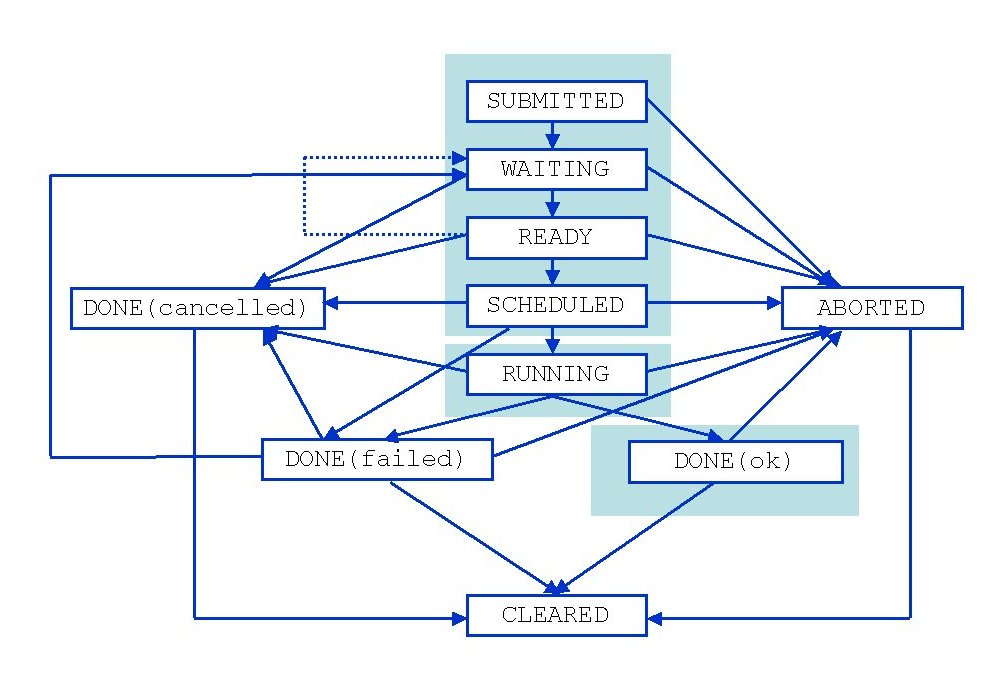
\includegraphics[width=.8\hsize]{job-state-diagram}
\caption{Job State Machine}
\label{job-state}
\end{figure}

Here below is provided a brief description of the meaning of each possible state a job/DAG can enter:

\begin{itemize}
\item {\it Submitted}: job is entered by the user to the User Interface but not yet transferred to Network Server for processing
\item {\it Waiting}: job has been accepted by NS and is waiting for Workload Manager processing or is being processed by WM Helper modules (e.g., WM is busy, no appropriate Computing Element (cluster) has been found yet, required dataset is not available, job is waiting for resource allocation).
\item {\it Ready}: job has been processed by WM and its Helper modules (especially, appropriate Computing Element has been found) but not yet transferred to the Computing Element (local batch system queue) via Job Controller and CondorC. This state does 
not exists for a DAG as it is not subjected to matchmaking (the nodes are) but passed directly to DAGMan.  
\item {\it Scheduled}: job is waiting in the queue on the Computing Element. This state also does not exists for a DAG as it is not directly sent to a CE (the node are). 
\item {\it Running}: job is running. For a DAG this means that DAGMan has started processing it.
\item {\it Done}: job exited or is considered to be in a terminal state by CondorC (e.g., submission to CE has failed in an unrecoverable way). 
\item {\it Aborted}: job processing was aborted by WMS (waiting in the Workload Manager queue or Computing Element for too long, over-use of quotas, expiration of user credentials, etc.).
\item {\it Canceled}: job has been successfully canceled on user request.
\item {\it Cleared}: output sandbox was transferred to the user or removed due to the timeout.
\end{itemize} 

Taken into account remarks about DAGs in the previous state description, the following figure~\ref{dag-state} represents instead the DAG 
life-cycle state machine:

\begin{figure}[htb]
\centering
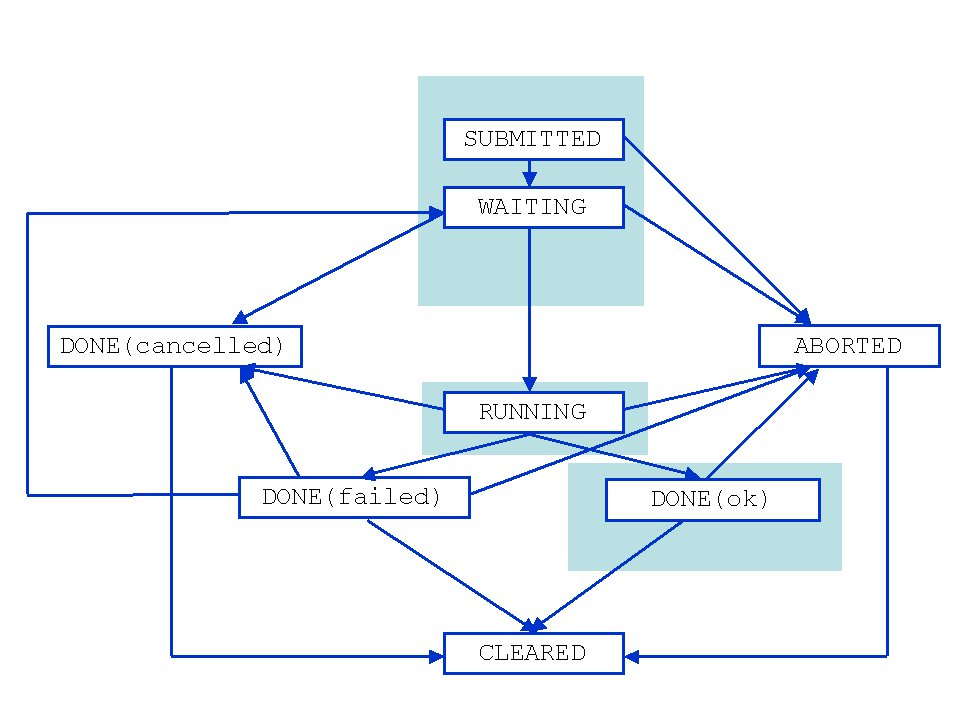
\includegraphics[width=.8\hsize]{dag-state-diagram}
\caption{DAG State Machine}
\label{dag-state}
\end{figure}

\newpage
 
\textbf{glite-job-output}

The glite-job-output command can be used to retrieve the output files of a job/DAG that has been submitted through the 
glite-job-submit command with a job description file including the OutputSandbox attribute. After the submission, 
when the job/DAG has terminated its execution, the user can download the files generated by the job/DAG and temporarily 
stored on the Resource Broker machine as specified by the OutputSandbox attribute, issuing the 
glite-job-output with as input the ID returned by the glite-job-submit. As a DAG does not have its own output sandbox, 
when the command is issues for such a request retrieves the output sandboxes of all the DAG nodes.

\textbf{glite-job-cancel}

This command cancels a job previously submitted using glite-job-submit. Before cancellation, it prompts the user 
for confirmation. The cancel request is sent to the Network Server that forwards it to the WM that fulfills it. 
It is not allowed to issue a cancel request for a node of a DAG: you have to cancel the whole DAG using the 
provided handle instead.


\medskip

The WMS-UI also provides three additional commands. They are: 

\begin{itemize}
   \item glite-job-logging-info $<$job\_Id$>$ (mostly useful for debugging purposes)
   \item glite-job-attach $<$job\_Id$>$ (for interactive jobs only)
   \item glite-job-get-chkpt $<$job\_Id$>$ (for checkpointable jobs only)
\end{itemize}


\textbf{glite-job-logging-info}

This command prints all the events related to a previously submitted job/DAG, that have been logged to the LB during 
request's lifetime by the WMS components that have handled it. The job/DAG logging-info request is sent
to the LB (Logging and Bookkeeping service) that provides the requested information. When issues for a DAG the 
command only displays events related to the DAG itself and not the ones of the nodes. 

\textbf{glite-job-attach}

This command attaches a listener to a previously submitted interactive job. This will make the job standard streams 
be re-directed to the command shell (or to a dedicated graphical window - if requested).

\textbf{glite-job-get-chkpt}

This command retrieves a checkpoint state of a a previously submitted checkpointable job. The retrieved state, that
is saved to a file on the WMS-UI machine, can be used later to re-submit either the same or another checkpointable 
job so that it will start its execution from the given state rather than from the beginning.

\smallskip
\subsection{The Job Identifier}

The Job (and DAG) Identifiers produced by the workload management software are of the form:

\smallskip
\begin{verbatim}
https://edt003.cnaf.infn.it:9000/NyIYrqE\_a8igk4f0CLXNKA
\end{verbatim}
\smallskip

The first part of the Id (\emph{https://edt003.cnaf.infn.it:9000} in the example above) is the endpoint URL of the 
LB server holding the job/DAG logging and bookkeeping information and this allows the WMS-UI to know which LB server has 
to be contacted for monitoring a given job/DAG. 
\smallskip
The second part (\emph{NyIYrqE\_a8igk4f0CLXNKA})  generated by the WMS-UI taking into account some client local information 
ensures instead grid-wide uniqueness of the identifier. 

    
\subsection{The Job Description File}

The key to the job submission and resource matching process is the JDL description file. This file describes 
the necessary inputs, generated outputs, and resource requirements of a job/DAG through the JDL 
(Job Description Language).

A typical example of a job description file is:

\smallskip
\begin{verbatim}
 [
   Type = "Job";
   JobType = "Normal";
   Executable = "myexe";
   StdInput = "myinput.txt";
   StdOutput = "message.txt";
   StdError = "error.txt";
   InputSandbox = {"/users/pacini/example/myinput.txt", 
                   "/users/pacini/example/myexe"};
   OutputSandbox = {"message.txt", "error.txt"};
   Requirements  = other.GlueCEInfoLRMSType == "PBS";
   Rank  = other.FreeCPUs;
 ]
\end{verbatim}
\smallskip

Such a JDL would make the \emph{myexe} executable be transferred on a remote CE whose queue is managed by the PBS batch 
system and be run taking the \emph{myinput.txt} file (also copied form the UI node) as input. The standard streams of the 
job are redirected on the worker node to file \emph{message.txt} and \emph{error.txt} and can be later retrieved on the 
WMS-UI by means of the \emph{glite-job-output} command. 


A simple example of DAG description, call it \emph{dag.jdl}, is instead:

\smallskip
\begin{verbatim}
 [
    Type = "dag";
    max_nodes_running = 10;
    VirtualOrganisation = "EGEE";
    nodes = [
      nodeA = [
        file ="/users/pacini/n1.jdl" ; 
      ];
      nodeB = [
        file ="/users/pacini/n2.jdl" ; 
      ];
      nodeB = [
        file ="/users/pacini/n3.jdl" ; 
      ];
      dependencies = {
        { nodeA, {nodeB, nodeC}}
      }
    ];
  ]
\end{verbatim}
\smallskip

where n1.jdl, n2.jdl and n3.jdl are in turn job descriptions representing the nodes of the DAG and the dependencies 
attributes states that \textit{nodeB} and \textit{nodeC} cannot start before \textit{nodeA} has been successfully executed. 
Also the DAGs are submitted through the \emph{glite-job-submit} command.

A detailed description of the available JDL attributes and of the rules for building correct JDL files is 
provided by the "JDL Attributes Specification" document ~\cite{jdl}.  

It is important to note note that the input and output sandboxes are intended for relatively small files 
(few megabytes) like scripts, standard input, and standard output streams.
If you are using large input files or generating large output files, you should instead directly read from or 
write to a storage element. As each submitting user is assigned by the WMS with a limited quota on the WMS 
machine disk, abuse of the input and output sandboxes will shortly make the quota fill-up and the WMS not accept 
further jobs submission for the given user. 

The parameters Requirements and Rank control the resource matching for the job. The expression given for the 
requirements specifies the constraints necessary for a job to run. In the example above, a site running PBS is 
required and the job will only be submitted to resources which satisfy this condition. If more than one resource 
matches the job requirements, then the rank is used to determine which is the most desirable resource i.e. the one 
to which the job is submitted (the higher the rank value the better is the resource). 
Both, the Requirements and the rank attributes, can be arbitrary expressions which use the parameters published 
by the resources in the Information System or directly to the ISM.
A DAG does not have its own requirements and ranking expressions: matchmaking is performed on the individual nodes 
Rank and Requirements.

\smallskip
\subsection{Commands Sequence}

This section reports an example of the sequence of steps that have to be performed to do a job submission and to monitor 
the submitted job.
 
Before using any of the WMS-UI commands it is necessary to have a valid proxy credential available on the WMS-UI
machine. You can create it using the \textit{voms-proxy-init} command or alternatively the \textit{grid-proxy-init} one. 
If you already have a valid proxy available on your machine just make the X509\_USER\_PROXY environment variable 
point to it.

In order to get a proxy certificates issued by VOMS ~\cite{voms-core} you should have in your home directory the file 
\$HOME/.glite/vomses containing a line as follows:

\smallskip
{\scriptsize{\verb!"EGEE" "kuiken.nikhef.nl" "15001" "/O=dutchgrid/O=hosts/OU=nikhef.nl/CN=kuiken.nikhef.nl" "EGEE" "22"!}}
\smallskip

or the corresponding line for your VO (ask your VO admin for that).


Make moreover sure you have in the directory \textit{\$HOME/.globus} your certificate/key pair, i.e. the following files:  

\smallskip

\begin{scriptsize}
\begin{verbatim}
usercert.pem
userkey.pem
\end{verbatim}
\end{scriptsize}
\smallskip

Note that file permissions are important: the two files must have respectively \textit{0600} and \textit{0400} permissions.  

Then you can issue the VOMS client command (you will be prompted for the pass-phrase):

\smallskip
\begin{scriptsize}
\begin{verbatim}

> voms-proxy-init --userconf vomses -voms EGEE
Your identity: /C=IT/O=INFN/OU=Personal Certificate/L=DATAMAT DSAGRD/CN=Fabrizio Pacini
Enter GRID pass phrase for this identity:
Creating temporary proxy ..................................... Done
/O=dutchgrid/O=hosts/OU=nikhef.nl/CN=kuiken.nikhef.nl
/C=NL/O=NIKHEF/CN=NIKHEF medium-security certification auth
Creating proxy ............................ Done
Your proxy is valid until Sat Mar  5 06:13:07 2005

> voms-proxy-info
VO              : EGEE
Valid from      : Mar  4 17:13:08 2005 GMT
Valid to        : Mar  5 05:13:08 2005 GMT

\end{verbatim}
\end{scriptsize}
\smallskip


Now you can start using the WMS-UI commands.
It is often useful to check the results of the resource matching before submitting a job. For this, one can use 
the \emph{glite-job-list-match} command. Given the JDL file it will return a ranked list of matching resources. 
The highest-ranked resource will appear first.

Take for example the following  JDL file, say \textit{ HelloWorld.jdl}:

\smallskip
\begin{verbatim}

 [
   Executable = "/bin/echo";
   Arguments = "Hello World";
   StdOutput = "message.txt";   StdError = "stderror";
   OutputSandbox = {"message.txt","stderror"};
   rank = -other.GlueCEStateEstimatedResponseTime;
   requirements = other.GlueCEStateStatus == "Production"; 
 ]

\end{verbatim}
\smallskip

you can get the list of available CEids and then submit as follows: 

\smallskip
\begin{scriptsize}
\begin{verbatim}

> glite-job-list-match HelloWorld.jdl
   
Selected Virtual Organisation name (from proxy certificate extension): EGEE   
Connecting to host edt003.cnaf.infn.it, port 7772

****************************************************
                    COMPUTING ELEMENT IDs LIST
The following CE(s) matching your job requirements 
have been found:

                            *CEId*
grid20.bo.ingv.it:2119/jobmanager-pbs-infinite
grid20.bo.ingv.it:2119/jobmanager-pbs-long
grid20.bo.ingv.it:2119/jobmanager-pbs-short
gridba2.ba.infn.it:2119/jobmanager-lcgpbs-infinite
gridba2.ba.infn.it:2119/jobmanager-lcgpbs-long
gridba2.ba.infn.it:2119/jobmanager-lcgpbs-short
gridit001.pd.infn.it:2119/jobmanager-pbs-infinite
gridit001.pd.infn.it:2119/jobmanager-pbs-long
gridit001.pd.infn.it:2119/jobmanager-pbs-short
****************************************************

\end{verbatim}
\end{scriptsize}
\smallskip

and once verified that you are happy with the matching resources, you cab actually submit the job:

\smallskip
\begin{scriptsize}
\begin{verbatim}

> glite-job-submit HelloWorld.jdl

Selected Virtual Organisation name (from proxy certificate extension): EGEE
Connecting to host edt003.cnaf.infn.it, port 7772
Logging to host edt003.cnaf.infn.it, port 9002

**************************************************************
                  JOB SUBMIT OUTCOME
The job has been successfully submitted to the Network Server.
Use glite-job-status command to check job current status. 
Your job identifier is:

- https://edt003.cnaf.infn.it:9000/NyIYrqE\_a8igk4f0CLXNKA

***************************************************************

\end{verbatim}
\end{scriptsize}
\smallskip


Note that this command returns the job identifier associated with this job. The job Id 
is the unique Grid Job Identifier, assigned from the WMS (Workload Management System) to every job in order to 
be able to identify it in clear and unique way all over the Grid system scope.

Passing the job id handle to the WMS commands you can follow-up the submitted job:

\smallskip
\begin{scriptsize}
\begin{verbatim}

> glite-job-status https://edt003.cnaf.infn.it:9000/NyIYrqE\_a8igk4f0CLXNKA

****************************************************************************
BOOKKEEPING INFORMATION:

Printing status info for the Job :
https://edt003.cnaf.infn.it:9000/NyIYrqE\_a8igk4f0CLXNKA
Current Status:Done (Success)
Exit code: 0
Status Reason: Job terminated successfully
Destination:   gridit001.pd.infn.it:2119/jobmanager-lcgpbs-infinite
reached on:Mon Sep 22 09:37:13 2003 CET
****************************************************************************
\end{verbatim}
\end{scriptsize}
\smallskip

States seen in the normal processing of jobs are: \textit{Submitted, Waiting, Ready, Running} and \textit{Done}. Abnormal 
execution usually ends with an Aborted status.

Once you have checked that the job has terminated its execution successfully (\emph{Done} status), i.e. the job has 
finished and the output has been pushed back to the WMS node, you can retrieve the output of your job to the 
WMS-UI machine as follows:

\smallskip
\begin{scriptsize}
\begin{verbatim}

> glite-job-output https://edt003.cnaf.infn.it:9000/NyIYrqE\_a8igk4f0CLXNKA

Retrieving files from host edt003.cnaf.infn.it

****************************************************************************
		JOB GET OUTPUT OUTCOME

Output sandbox files for the job:
- https://edt003.cnaf.infn.it:9000/NyIYrqE\_a8igk4f0CLXNKA
have been successfully retrieved and stored in the directory:
/tmp/jobOutput/mrossi__NyIYrqE\_a8igk4f0CLXNKA

****************************************************************************
\end{verbatim}
\end{scriptsize}
\smallskip

where \textit{/tmp/jobOutput} is the output storage path set in you configuration file and 
\textit{mrossi\_\_NyIYrqE\_a8igk4f0CLXNKA} is a directory name built concatenating your current OS user-name and
the job Id unique string. 

Use the \emph{--dir} option if you want the output to be saved in a location different from \textit{/tmp/jobOutput}.  

Handling the job identifiers directly quickly becomes tedious. To avoid this, you can make the \emph{glite-job-submit} 
command append the job Id to a named file using the \emph{--output} option. 
On the other side, the WMS-UI commands which take job identifiers as an argument accept also the \emph{--input} option 
which allows the job identifier to be read from a file.
It is possible anyway to retrieve the status information for all jobs you have submitted  for a given VO by using 
the \emph{--all} option of the  \emph{glite-job-status} command: 

\smallskip
\begin{scriptsize}
\begin{verbatim}

> glite-job-status --all 

\end{verbatim}
\end{scriptsize}
\smallskip


If something is not going as expected with your job, e.g. it is \textit{Aborted} or it does not reach the \textit{Done} 
status you can try the \emph{glite-job-logging-info} command to inspect the job related events. Assuming your job 
identifier is e.g. \textit{https://gundam.cnaf.infn.it:9000/WkyitIdNTR0C9adOcBPhwg}, you can type:

\smallskip
\begin{scriptsize}
\begin{verbatim}

> glite-job-logging-info https://gundam.cnaf.infn.it:9000/WkyitIdNTR0C9adOcBPhwg

**********************************************************************
LOGGING INFORMATION:

Printing info for the Job : https://gundam.cnaf.infn.it:9000/WkyitIdNTR0C9adOcBPhwg
 
        ---
Event: RegJob
- source                  =    UserInterface
- timestamp               =    Fri Mar  4 18:05:28 2005 CET
        ---
Event: Transfer
- destination             =    NetworkServer
- result                  =    START
- source                  =    UserInterface
- timestamp               =    Fri Mar  4 18:05:29 2005 CET
        ---
Event: Transfer
- destination             =    NetworkServer
- result                  =    OK
- source                  =    UserInterface
- timestamp               =    Fri Mar  4 18:05:32 2005 CET
        ---
Event: Accepted
- source                  =    NetworkServer
- timestamp               =    Fri Mar  4 18:05:23 2005 CET
        ---
....

\end{verbatim}
\end{scriptsize}
\smallskip

to check if there was a problem within a certain WMS component and eventually cancel it with :

\smallskip
\begin{scriptsize}
\begin{verbatim}

> glite-job-cancel https://gundam.cnaf.infn.it:9000/SpLbPbMpftBSnCr0WwJmZA

Are you sure you want to remove specified job(s)? [y/n]n :y

=============================  glite-job-cancel Success  ===========================
 The cancellation request has been successfully submitted for the following job(s):

 - https://gundam.cnaf.infn.it:9000/SpLbPbMpftBSnCr0WwJmZA

====================================================================================

\end{verbatim}
\end{scriptsize}
\smallskip

\subsubsection {DAGs}

DAG submission can be accomplished through the same commands used for simple jobs. 
If for example you want to submit the DAG defined above, \emph{dag.jdl}, once you have 
completed the proxy preparation steps, just issue the following command: 

\smallskip
\begin{scriptsize}
\begin{verbatim}

> glite-job-submit dag.jdl 

Selected Virtual Organisation name (from proxy certificate extension): EGEE
Connecting to host gundam.cnaf.infn.it, port 7772
Logging to host gundam.cnaf.infn.it, port 9002


**************************************************************************************
                               JOB SUBMIT OUTCOME
 The dag has been successfully submitted to the Network Server.
 Use glite-job-status command to check job current status. Your dag identifier is:

 - https://gundam.cnaf.infn.it:9000/AhM4clHKVD1VMOMVrdkCZw


**************************************************************************************
\end{verbatim}
\end{scriptsize}


and then monitor it by means of:


\smallskip
\begin{scriptsize}
\begin{verbatim}

> glite-job-status https://gundam.cnaf.infn.it:9000/AhM4clHKVD1VMOMVrdkCZw


*************************************************************
BOOKKEEPING INFORMATION:

Status info for the Job : https://gundam.cnaf.infn.it:9000/AhM4clHKVD1VMOMVrdkCZw
Current Status:     Ready 
Status Reason:      unavailable
Destination:        dagman
Submitted:          Mon Mar  7 17:25:22 2005 CET
*************************************************************

- Nodes information for: 
    Status info for the Job : https://gundam.cnaf.infn.it:9000/ayNofwCnlusD68s3qQvFEA
    Current Status:     Submitted 
    Submitted:          Mon Mar  7 17:25:08 2005 CET
    Parent Job:         https://gundam.cnaf.infn.it:9000/AhM4clHKVD1VMOMVrdkCZw
*************************************************************
    
    Status info for the Job : https://gundam.cnaf.infn.it:9000/9FfFXd7UIWuoPSlyqMVZNQ
    Current Status:     Submitted 
    Submitted:          Mon Mar  7 17:25:08 2005 CET
    Parent Job:         https://gundam.cnaf.infn.it:9000/AhM4clHKVD1VMOMVrdkCZw
*************************************************************
    
    Status info for the Job : https://gundam.cnaf.infn.it:9000/wlgiicvWUe6Br7nbjIxcnQ
    Current Status:     Submitted 
    Submitted:          Mon Mar  7 17:25:08 2005 CET
    Parent Job:         https://gundam.cnaf.infn.it:9000/AhM4clHKVD1VMOMVrdkCZw
*************************************************************

\end{verbatim}
\end{scriptsize}
\smallskip

As you can see the \emph{glite-job-status} command shows in this case information about the DAG
itself and all its nodes. Nodes can be also followed-up singularly by picking their job identifiers.

The \emph{glite-job-logging-info} returns instead only the events related to the DAG. Nodes logging information
have to be requested explicitly specifying the node Id. 

The \emph{glite-job-output} can be used for a DAG to request the retrieval of the output sandboxes of all its nodes. 

The \emph{glite-job-cancel} commands can be used for a DAG to request cancellation of the whole DAG whilst cannot be 
called for a single DAG node.  


\subsection {Long Lived Jobs}
\label{longjob}

It is possible that long jobs may outlive the validity of the initial proxy; if so and the proxy 
is not renewed, the job will die prematurely. To avoid this the workload management software allows 
the proxy to be renewed automatically if your credentials are managed by a MyProxy server.

To use the automatic proxy renewal mechanism, first register a proxy with the MyProxy server using 
the command

\smallskip
\verb!myproxy-init -s <server> -t <hours>  -d -n!
\smallskip

where \emph{server} is the MyProxy server address, \emph{hours} is the number of hours the proxy should be valid on the 
server.

As this proxy is only copied to the server, you will need to create a local short-lived proxy using 
voms-proxy-init as explained previously, to do the job submissions. The Workload Manager will 
retrieve renewed proxies from the MyProxy server for jobs which need and request them. 
The need for proxy renewal has to be explicitly specified in the JDL of the job/DAG through the 
\emph{MyProxyServer} attribute, e.g.:

\smallskip
\begin{verbatim}
MyProxyServer = "skurut.ics.muni.cz";
\end{verbatim}
\smallskip


Information about your stored proxy can be obtained via the command

\smallskip
\verb!myproxy-info -s <server> -d!
\smallskip

and the proxy can be removed with

\smallskip
\verb!myproxy-destroy -s <server> -d.!
\smallskip

Once the proxy is removed from the server, running jobs will no longer receive renewed credentials.


\subsection{Specifying Job Requirements}

By specifying job requirements, the user can steer the job to sites which have the resources 
necessary to run the job correctly. Incompletely specifying the requirements may cause the job 
to fail, wasting both the resources and the user's time.

The request requirements are specified through the \emph{Requirements} attribute in the JDL 
description of the job. The value of this attribute is a boolean expression which specifies the 
necessary constraints. Nearly the full set of C operators and syntax are supported.

The values (or variables) which can be used in the requirements expression can be found by looking 
at the Computing Element attributes in the BDII or subscribing to the CE Monitor notification service.
The current Glue Schema used for publishing CE information is however available at:
\url{http://www.cnaf.infn.it/~sergio/datatag/glue/index.htm}. Most of the attributes are 
self-explanatory.

For example to express that a job requires at least 25 minutes of CPU time and 100 minutes of real 
time, the expression:

\smallskip
{\scriptsize{
\verb!Requirements = other.GlueCEPolicyMaxCPUTime >= 1500 && other.GlueCEPolicyMaxWallClockTime >= 6000;!
}}
\smallskip


would limit the matching to viable sites. The times are given in seconds. 
Note that the attribute names are prefixed with \textit{other.}; this is a remnant of the Class-Ads syntax on 
which JDL is based indicating the the prefixed attribute has to be searched in the counterpart class-ad (i.e. the 
one describing the resource). Note also that the values are not quoted. Using quotes around a numeric value 
will result in a string comparison which will produce an erroneous match (or none at all).

The \textit{GlueHostApplicationSoftwareRunTimeEnvironment} is usually used to describe application software 
packages which are installed on a site. For example:

\smallskip
{\scriptsize{
\verb!Requirements  = Member(other.GlueHostApplicationSoftwareRunTimeEnvironment ,"ALICE-3.07.01");!
}}
\smallskip

will choose a site with the ALICE-3.07.01 tag defined. The \textit{GlueHostApplicationSoftwareRunTimeEnvironment} 
is a multi-valued attribute and evaluates to a list. The class-ad \textit{Member} function returns true if the given 
value is in the list.

The available built-in class-ad functions that can be used for building the requirements expression are 
described in ~\cite{jdl-lang}.

Occasionally, one may wish to exclude or include a site manually. Forcing a job to a site can be 
accomplished with the \emph{--resource} option of the glite-job-submit command. However, this 
entirely bypasses the matchmaking process and will not produce the \emph{.BrokerInfo} file, i.e. the 
file generated during the matchmaking phase, that is sent on the WN and contains data location 
information that can be useful for the job at run time. You can use instead a clause like:

\smallskip
{\scriptsize{
\verb!Requirements = other.GlueCEUniqueID == "ccgridli03.in2p3.fr:2119/jobmanager-bqs-A";!
}}
\smallskip
  
to do the same thing. More interestingly one can select or exclude a site:

\smallskip
\begin{scriptsize}
\begin{verbatim}   
Requirements  = RegExp(".*nikhef.*",other.GlueCEUniqueID);
Requirements  = (!(RegExp(".*nikhef.*",other.GlueCEUniqueID)));
\end{verbatim}
\end{scriptsize}
\smallskip


which cannot be accomplished with the --resource option. Note that the JDL is very picky about the 
logical not syntax. 

In the WMS-UI configuration file (\$GLITE\_LOCATION/etc/glite\_wmsui\_cmd\_var.conf) there is a 
requirements clause which is added to all JDL files by default. This is 

\smallskip
\begin{scriptsize}
\begin{verbatim}   
other.GlueCEStateStatus == "Production" ;
\end{verbatim}
\end{scriptsize}
\smallskip

If you have provided an expression for the requirements attribute in the JDL, the one specified in 
the configuration file is added (in AND) to the existing one. 

As a DAG does not have its own requirements, what stated in this section applies to the DAG nodes descriptions. 



\subsection{Ranking Resources}

If more than one resource matches the specified requirements, then the highest-ranked resource will
be used. If the Rank attribute is not specified in the user's JDL description, then

\smallskip
\begin{scriptsize}
\verb!Rank = - other.GlueCEStateEstimatedResponseTime ;!
\end{scriptsize}
\smallskip

is added by default by the WMS-UI (as specified in the WMS-UI configuration file).The traversal time is 
the expected time in seconds that a job will take to begin executing at the site from the it has 
entered the batch system queue.

This ranking is not always ideal, and the user may wish to choose some other criteria for the 
ranking. For example,

\smallskip
\begin{scriptsize}
\verb!Rank = other.GlueCEStateFreeCPUs ;!
\end{scriptsize}
\smallskip

will make the WMS choose the site with the largest number of free CPUs. The rule to remember is that 
the larger the rank, the more desirable the resource is. If more than one site has exactly the same 
rank, then the one which is used is chosen randomly by the RB.

As a DAG does not have its own rank, what stated in this section applies to the DAG nodes descriptions. 
